
	Es importante recalcar que la ganancia de Kalman $K_k$ es distinta para cada instante $k$. Cuando el sistema es variante en el tiempo, el filtro se adapta a las condiciones de dinámica y ruido instante a instante. Por otro lado, cuando el sistema es invariante en el tiempo puede demostrarse que tanto la matriz $K_k$, como la matriz $P_k$, convergen para tiempo infinito. Es decir:
	
	\begin{equation*}
		K_k \longrightarrow K
	\end{equation*}
	
	\begin{equation*}
		P_k \longrightarrow P
	\end{equation*}
	
	para $k \rightarrow \infty$. Dichas matrices pueden computarse mediante ecuaciones aritméticas discretas de Riccati (DARE). Es decir, $P$ debe cumplir:
	
	\begin{equation*}
		P = A P A^{*} - A P C^{*} (R + C P C^{*})^{-1} C P A + B Q B^{*}
	\end{equation*}
	
	Por otro lado la ganancia de Kalman puede calcularse como:
	
	\begin{equation*}
		K = P C^{*} (R + C P C^{*})^{-1}
	\end{equation*}
	
	Dadas estas matrices, surge la posibilidad de implementar una modificación al algoritmo de Kalman para que en lugar de utilizar las matrices calculadas instante a instante siempre utilice las matrices a las que va a converger, suponiendo que el sistema es invariante en el tiempo. Dicho algoritmo tiene la ventaja de que posee menos procesamiento en tiempo real, dado que las matrices $K$ y $P$ pueden computarse en tiempo de compilación y guardarse fijas en la memoria. Este algoritmo no será óptimo, pero puede demostrarse que la versión modificada convergerá a la versión original con rapidez exponencial, siendo más los beneficios que trae que los inconvenientes. El objetivo de este punto es comparar las dos variantes y demostrar lo expuesto. En la figura \ref{fig:ej3f_cov} podemos ver el resultado de la estimación. En linea punteada azul puede verse que la estimación del algoritmo modificado comienza desviada de la trayectoria, pero rapidamente converge a la misma. 

	\begin{figure}[H]
		\centering
		%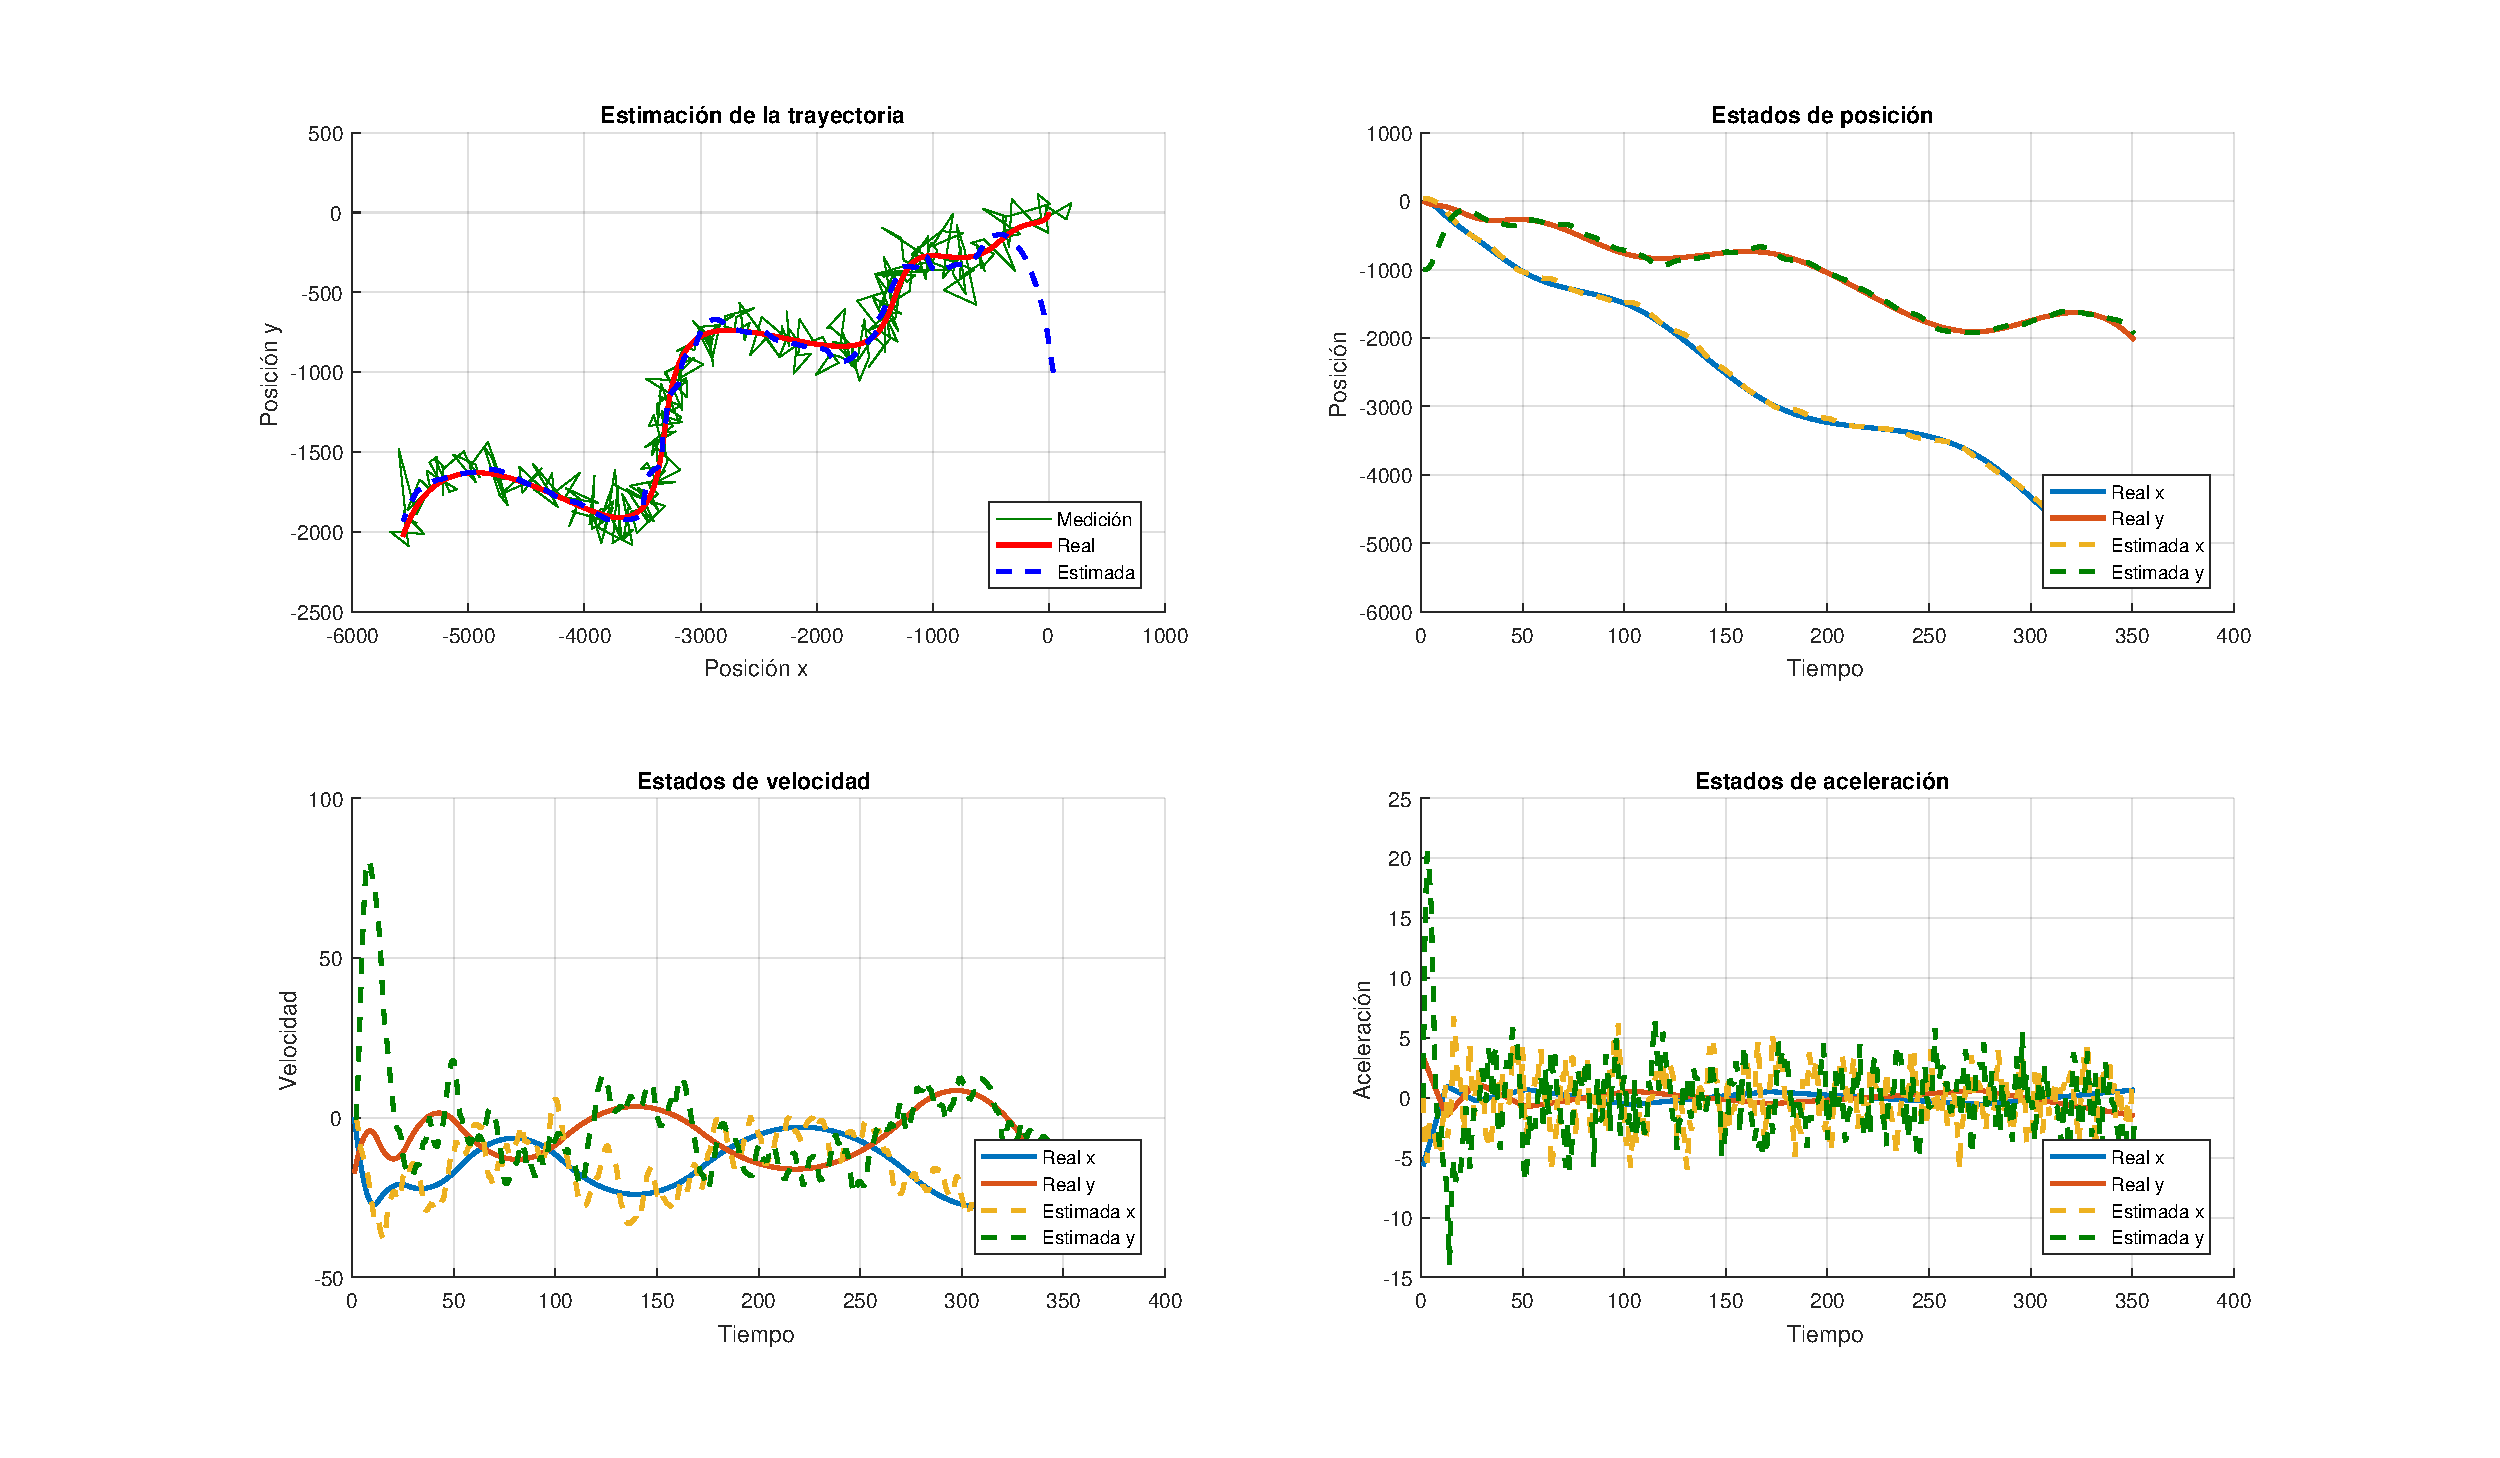
\includegraphics[width=1.0\textwidth,keepaspectratio]{Figuras/graf_ej5.pdf}
		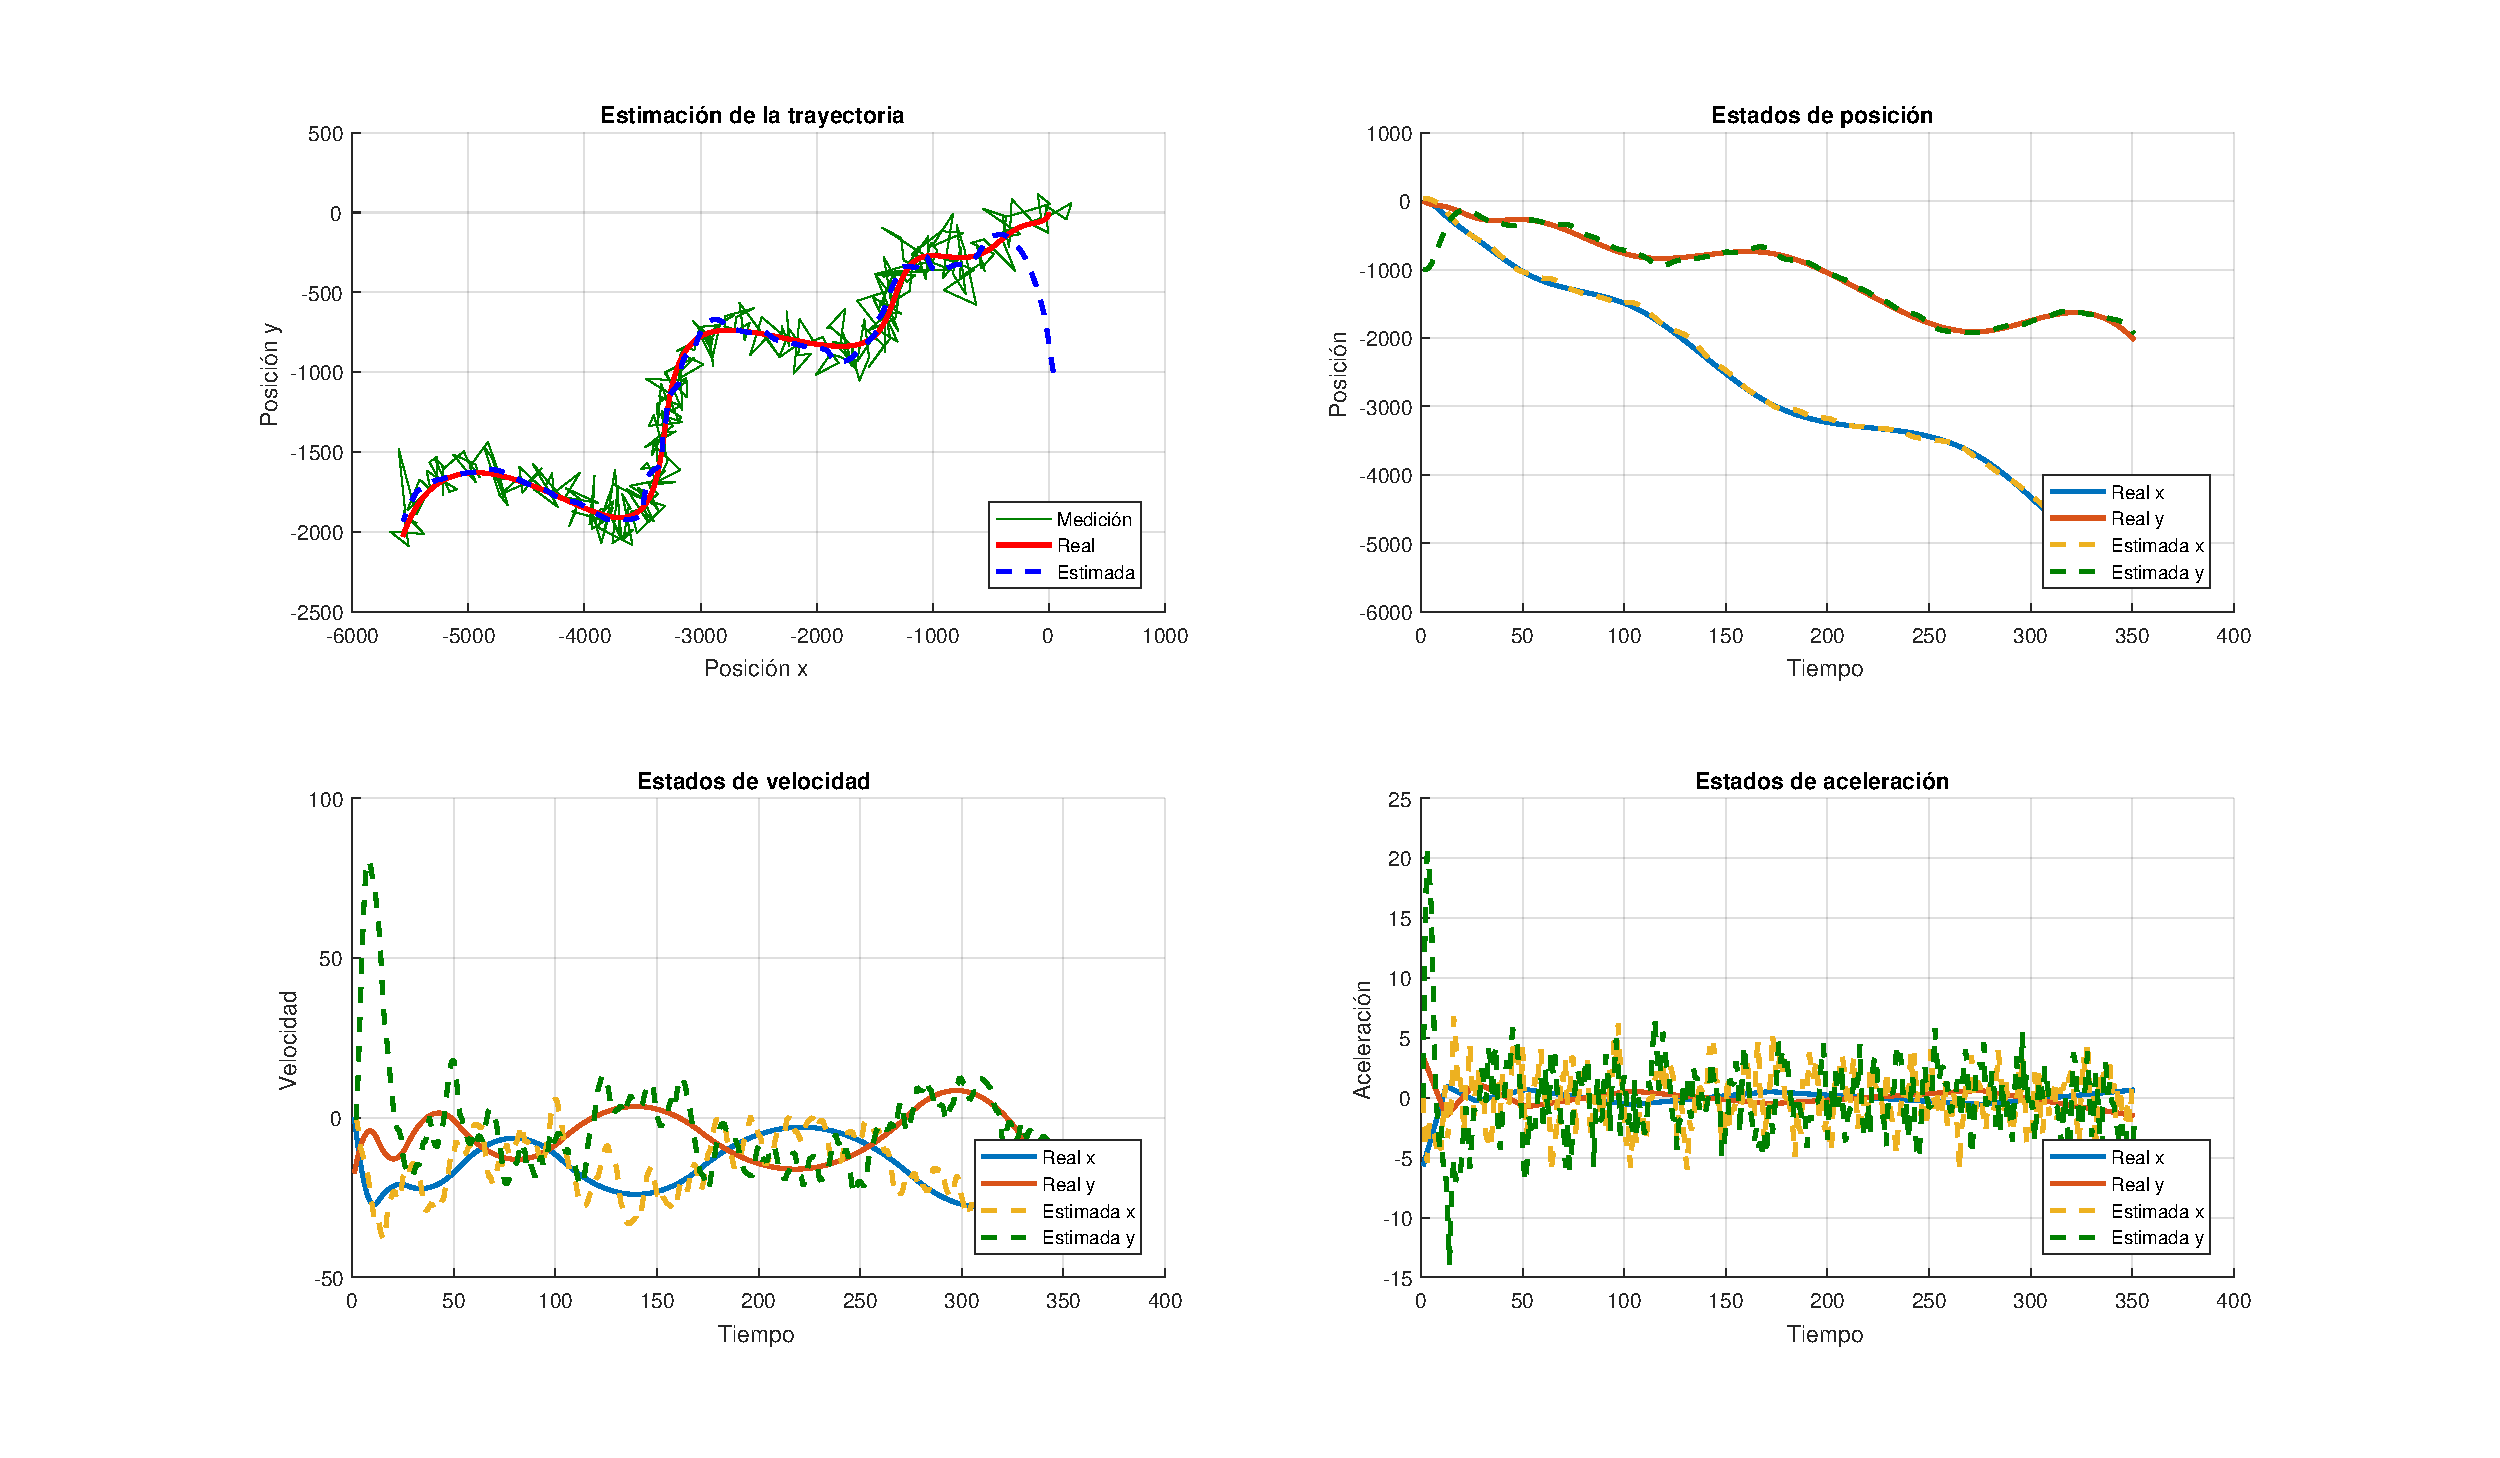
\includegraphics[scale=0.5,trim={6,5cm 0 0 0}]{Figuras/graf_ej5.pdf}
		\caption{Estimación de Trayectoria}
		\label{fig:ej6_cov}
	\end{figure}
	
	%Esta otra figura no se a que corresponde.
	%\begin{figure}[H]
	%	\centering
	%	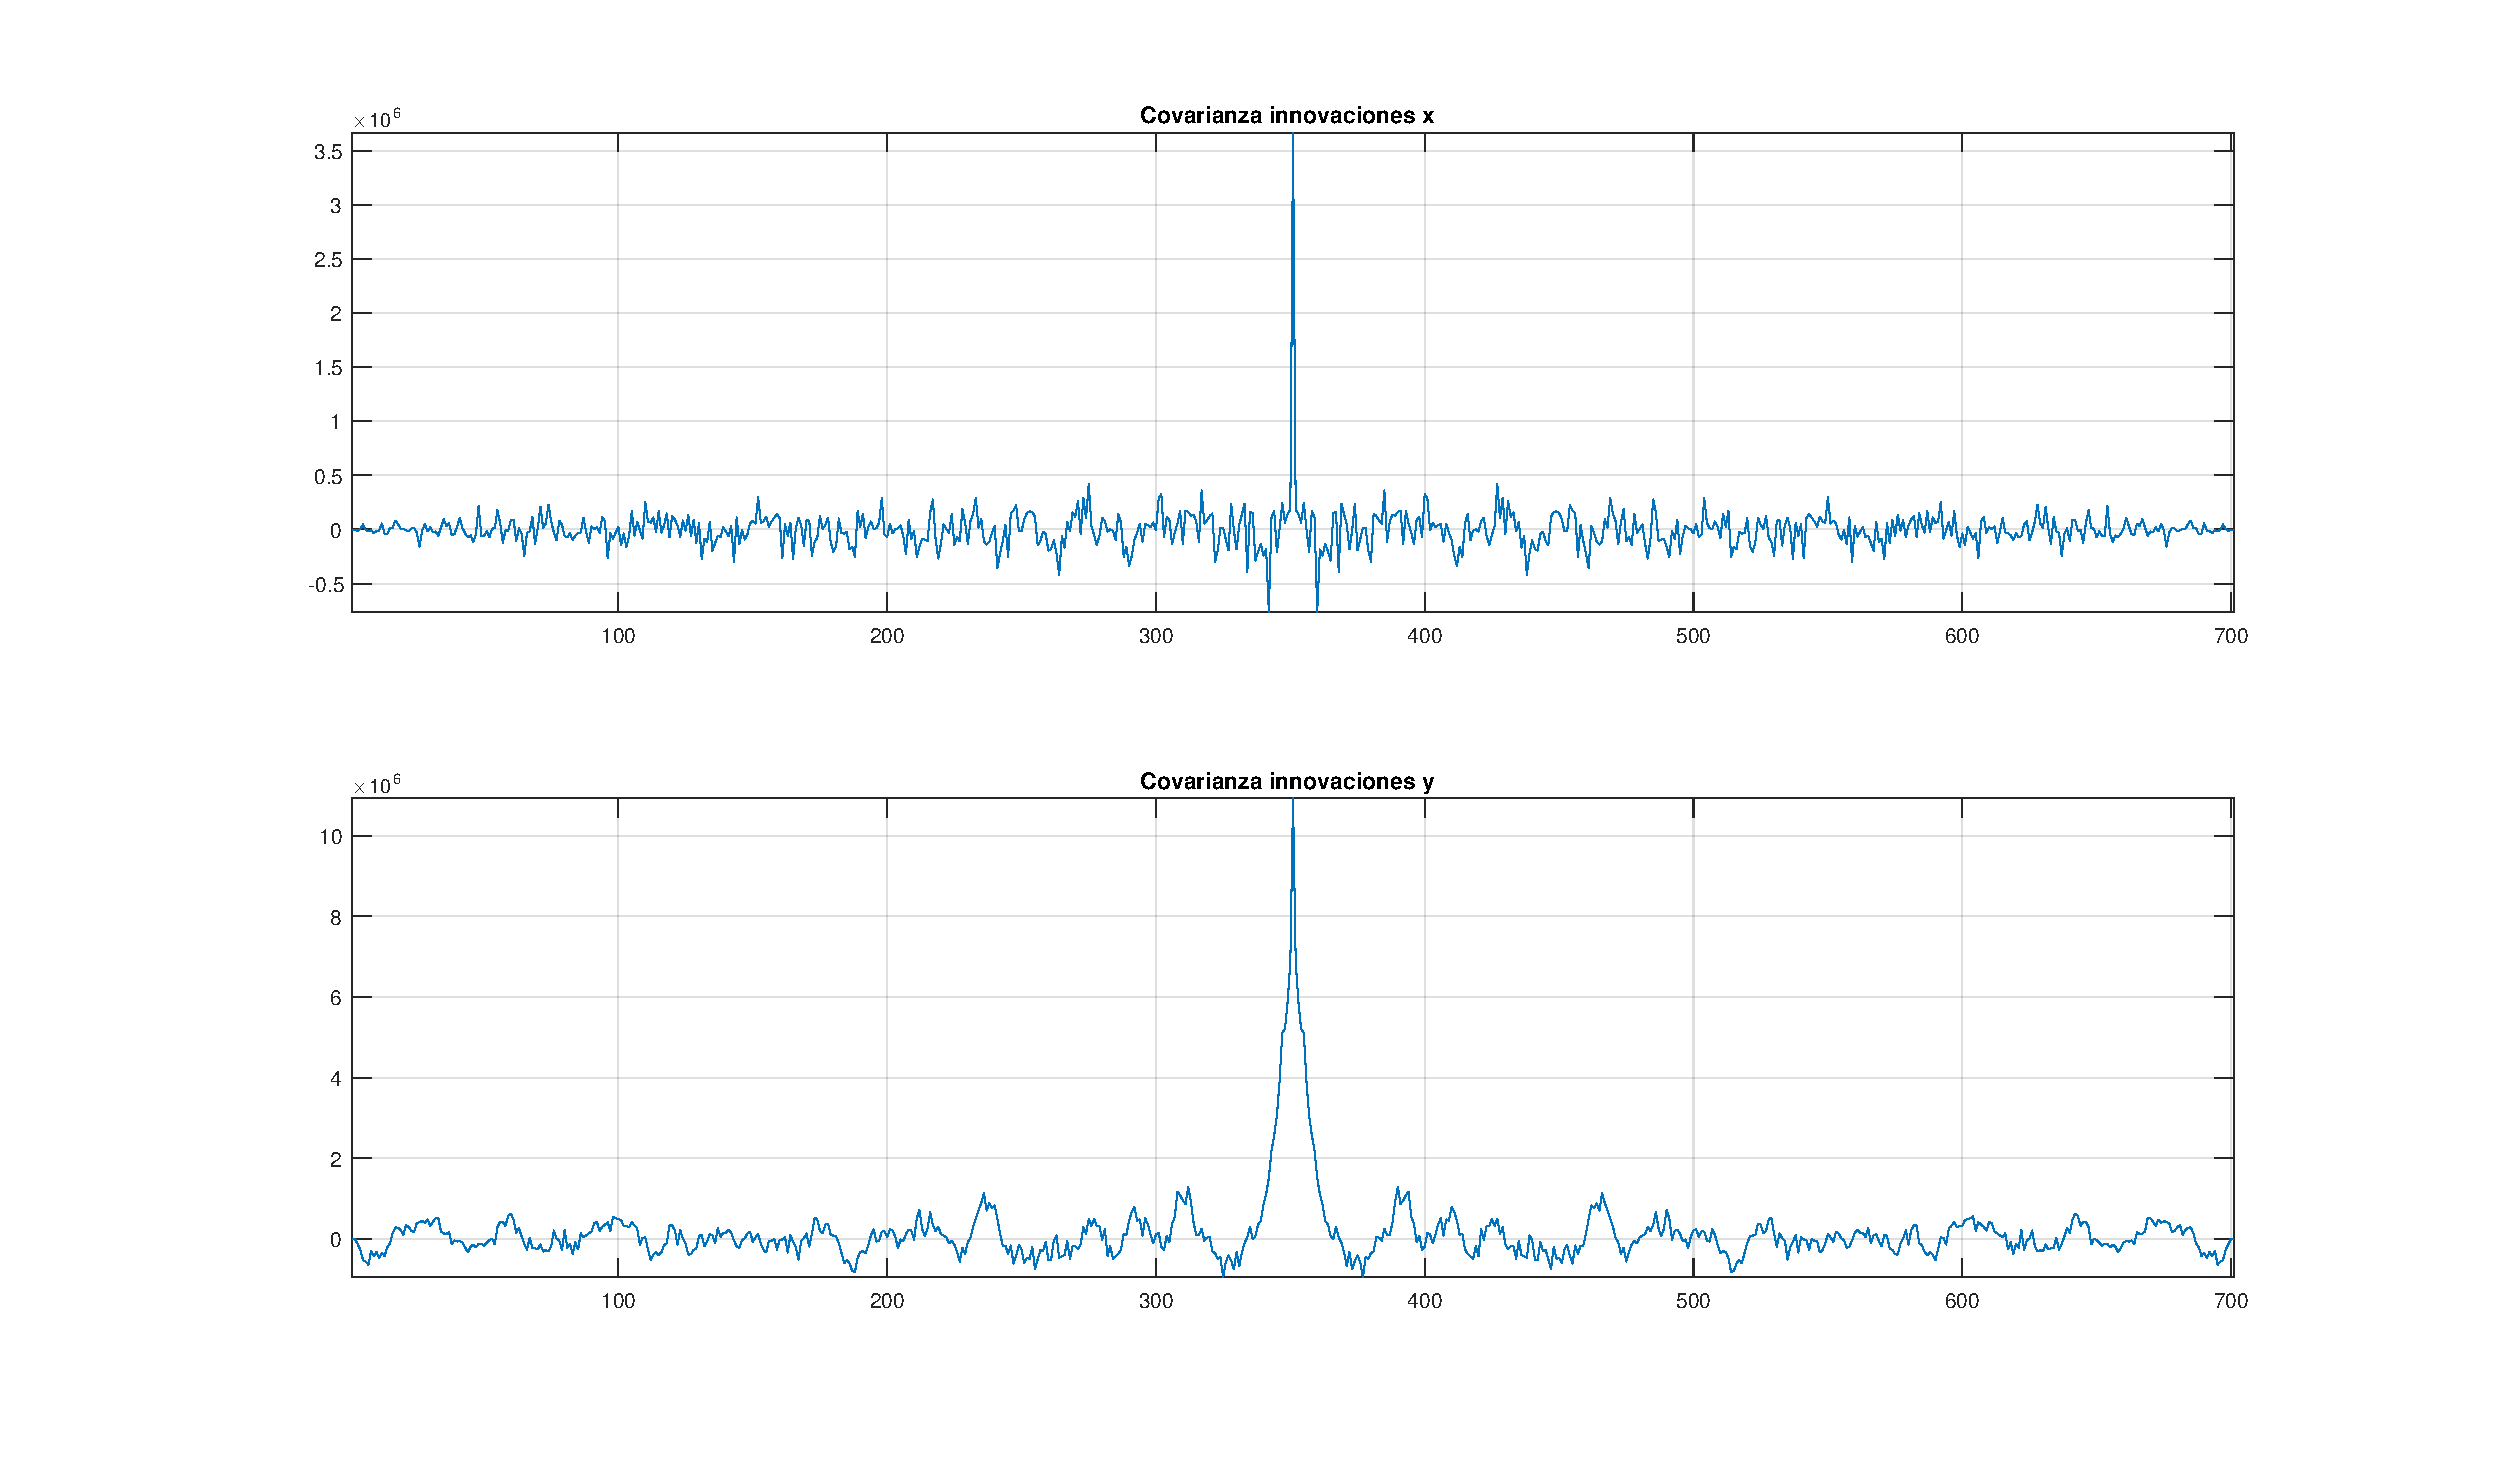
\includegraphics[width=1.0\textwidth,keepaspectratio]{Figuras/covinn_ej5.pdf}
	%	\caption{Correlación De Innovaciones}
	%	\label{fig:ej6_cov}
	%\end{figure}
	
	\subsection{Script}

	A continuación incluimos el script que realiza la estimación.
	
	%\lstinputlisting[]{../Octave/EJ5.m}
